\noindent Өнөөдрийн хичээлээр бид дараалалын хязгаарын тодорхойлолт, жишээ болон функцийн хязгаарын гол чанаруудтай танилцана. Эдгээр чанарууд нь өрөөсгөл хязгаар болон төгсгөлгүйд тэмүүлэх үед ч мөн адил үнэн байдаг.

\section{Дарааллын хязгаар}
Дараалал нь $f:\N\to\R$ функц тул  $x\to+\infty$ үед л хязгаар тодорхойлогдох боломжтой.\,
\begin{definition}[Дараалалын хязгаар]
 $ a_1, a_2, a_3, \ldots, a_n, \ldots$ бодит тоон дараалал байг. \\
Хэрэв дурын $\varepsilon>0$  тоо авах бүрт  
$$n>\delta \text{ байх бүх } n \text{ натурал тооны хувьд } |a_n-E|<\varepsilon$$
нөхцлийг хангах $\delta>0$ тоо олдож байвал $E$ тоог $a_n$ дараалалын  хязгаар гээд $$\lim\limits_{n\to  \infty}a_n=E$$ гэж бичнэ.   Хэрэв дараалал төгсгөлөг $E$ хязгаартай бол нийлдэг дараалал, бусад үед сарнидаг дараалал гэнэ.
\end{definition} 
\begin{example}[Төгсгөлөг хязгаартай дараалал]
$a_n = \dfrac{n}{n+1}$ дараалал өгөгдөв.  \[
\lim_{n\to\infty}\frac{n}{n+1}=1.
\] харуулая.
\[
\frac{n}{n+1}=1-\frac{1}{n+1}
\]  байна.
Дурын $\varepsilon>0$ хувьд $\delta=\frac{1}{\varepsilon}$ гэе. Хэрэв $n>1+\delta=\frac{1}{\varepsilon}+1>\dfrac{1}{\varepsilon}$ бол $\dfrac{1}{n+1}<\varepsilon$ байна. Иймд 
\[
\left|\frac{n}{n+1}-1\right| =\left|\frac{n-(n+1)}{n+1}\right|=\frac{1}{n+1}< \varepsilon.
\]
Иймд
\[
\lim_{n\to\infty}\frac{n}{n+1}=1
\] батлагдав.
\end{example}
\begin{example}[Төгсгөлгүй рүү тэмүүлэх дараалал]
$a_n = n$ дараалал өгөгдөв.  
Дурын $M>0$ бодит тоонд $\delta=M$ гэж авъя. Тэгвэл $n>\delta$ үед $a_n=n>M$.  
Иймд
\[
\lim_{n\to\infty} n = +\infty.
\]
\end{example}



\begin{example}[Хязгаар оршдоггүй дараалал]
$a_n = (-1)^n$ дараалал нь 
\[
\lim_{n\to\infty} (-1)^n \quad \text{оршихгүй}.
\]
\end{example}
\begin{prof}
Эсрэгээр нь $\{a_n\}$ дараалалын хязгаар $L\in\mathbb{R}$ оршино гэж үзье. 
Нийлэхийн тодорхойлолтоор дурын $\varepsilon>0$ тооны хувьд $\exists\,N\in\mathbb{N}$ ба $n>N$ үед 
\[
|a_n-L|<\varepsilon
\]
байх ёстой.

Одоо $\varepsilon=1$ гэж авъя. Тэгвэл $\exists\,N$, $n>N$ үед $|a_n-L|<1$ байх ёстой.
 $a_n$-ийн тэгш ба сондгой индексүүдийг ялгаж авч үзье:
\[
a_{2k}=1,\qquad a_{2k+1}=-1\quad (k\in\mathbb{N}).
\]
\textbf{(i) Хэрэв $L> 0$} бол сондгой бүх $n> N$-д $a_n=-1$ тул
\[
|a_n-L|=|-1-L|=1+L\ge 1,
\]
ингэснээр $|a_n-L|<1$ нөхцөл зөрчлөгдөнө.

\textbf{(ii) Хэрэв $L\le 0$} бол тэгш бүх $n> N$-д $a_n=1$ тул
\[
|a_n-L|=|1-L|=1-L\ge 1,
\]
дахиад л $|a_n-L|<1$ нөхцөл зөрчинө.

Харин \textbf{$L$ нь $>0$ эсвэл $\le 0$ хоёрын нэг} байх тул аль ч тохиолдолд зөрчил гарч байна. 
Иймээс анхны таамаг (\(L\) хязгаар оршино) буруу. Тэгэхээр
\[
\lim_{n\to\infty}(-1)^n \ \text{оршихгүй}.
\]
\end{prof}
\chapter{Хязгаарын тухай теоремүүд }

\begin{theorem}[Хязгаар ганц байх тухай]\label{uniqlim}
$f:X\to\R$ функц, $x\to a$ байг. Хэрэв $\displaystyle\lim_{x\to a} f(x)$ хязгаар оршин байвал цор ганц байна. Өөрөөр хэлбэл хэн, хаана, ямар аргаар бодсон ч ижил утгатай.
\end{theorem}

\begin{prof}
Эсрэгээр нь $\lim_{x\to a}f(x)=b_1$ болон $\lim_{x\to a}f(x)=b_2$ гэсэн хоёр өөр хязгаар ($b_1>b_2$) оршин байдаг гэж үзье.

$\varepsilon=\dfrac{b_1-b_2}{3}$ авбал $b_2+\varepsilon=b_1-2\varepsilon<b_1-\varepsilon$ байна. Иймд $\emptyset=(b_1-\varepsilon, b_1+\varepsilon)\cap (b_2-\varepsilon,b_2+\varepsilon)$ болов.

Хязгаарын тодорхойлолтоор $\exists\,\delta_1>0$ ба, $|x-a|<\delta_1$ үед $|f(x)-b_1|<\varepsilon$; мөн $\exists\,\delta_2>0$ ба, $|x-a|<\delta_2$ үед $|f(x)-b_2|<\varepsilon$. $|x_0-a|<\min(\delta_1,\delta_2)$ бүхий $x_0$ сонговол
\[
b_2-\varepsilon<f(x_0)<b_2+\varepsilon<b_1-\varepsilon<f(x_0)<b_1+\varepsilon,
\]
гэж зөрчил гарна. Иймд $b_1=b_2$.
\end{prof}
\begin{theorem}[Хязгаарын энгийн чанарууд]\label{conslim}
$c,a$ тогтмол тоонууд, $x\to a$ байг. Дараах тэнцэтгэлүүд үнэн:
\begin{description}[leftmargin=2em]
  \item[(P1)] $\displaystyle\lim_{x\to a} c = c$,
  \item[(P2)] $\displaystyle\lim_{x\to a} x = a$.
\end{description}
\end{theorem}

\begin{prof}
(P1) $f(x)\equiv c$. Дурын $\varepsilon>0$ үед ямар ч $\delta>0$ дээр $|f(x)-c|=0<\varepsilon$, тиймээс $\lim_{x\to a}c=c$.

(P2) $f(x)=x$. Дурын $\varepsilon>0$ үед $\delta=\varepsilon$ гэж авбал $|x-a|<\delta$ үед $|f(x)-a|=|x-a|<\varepsilon$, тиймээс $\lim_{x\to a}x=a$.
\end{prof}
\begin{theorem}[Хязгаар ба үйлдлүүд]\label{aritlim}
$f,g:X\to\R$, $x\to a$, $A,B,C\in\R$ байг. Хэрэв $$\displaystyle\lim_{x\to a} f(x)=A \text{ ба } \displaystyle\lim_{x\to a} g(x)=B$$ бол:
\begin{description}[leftmargin=2em]
  \item[(P3)] $f$ нь $(a-p,a+p)\cap X$ олонлог дээр зааглагдсан байх  $\exists\,p>0$;
  \item[(P4)] $\displaystyle\lim_{x\to a}f(x)\pm g(x)=A\pm B$;
  \item[(P5)] $\displaystyle\lim_{x\to a} C\,g(x)=CB$, \quad $\displaystyle\lim_{x\to a} f(x)g(x)=AB$;
  \item[(P6)] Хэрэв $B\neq 0$ бол $\displaystyle\lim_{x\to a}\dfrac{f(x)}{g(x)}=\dfrac{A}{B}$.
\end{description}
\end{theorem}

\begin{prof}
(P3) Хязгаар оршин байвал $\exists\,p>0$ ба, $|x-a|<p$ үед $|f(x)-A|<1$ болно. Иймээс $A-1<f(x)<A+1$ болж $(a-p,a+p)\cap X$ дээр зааглагдсан.

(P4) Хязгаарын тодорхойлолтоор:
\begin{align*}
&\forall\,\varepsilon_1>0,\;\exists\,\delta_1>0\text{ тийм, }|x-a|<\delta_1\Rightarrow |f(x)-A|<\varepsilon_1,\\
&\forall\,\varepsilon_2>0,\;\exists\,\delta_2>0\text{ тийм, }|x-a|<\delta_2\Rightarrow |g(x)-B|<\varepsilon_2.
\end{align*}

Дурын $\varepsilon>0$ өгөгдсөн байг.  
Бид $\varepsilon_1=\varepsilon_2=\dfrac{\varepsilon}{2}$ гэж авъя.

Тэгвэл:
\[
|f(x)-A|<\frac{\varepsilon}{2},\qquad |g(x)-B|<\frac{\varepsilon}{2}.
\]
Одоо $\delta=\min(\delta_1,\delta_2)$ гэж авбал $|x-a|<\delta$ үед дээрх хоёр тэнцэтгэл биш хоёулаа биелнэ.  
Тэгвэл
\begin{align*}
|(f(x)\pm g(x))-(A\pm B)|
&=|(f(x)-A)\pm(g(x)-B)|\\
&\le |f(x)-A|+|g(x)-B|\\
&<\frac{\varepsilon}{2}+\frac{\varepsilon}{2}=\varepsilon.
\end{align*}
Иймд хязгаарын тодорхойлолтоор
\[
\lim_{x\to a}\bigl(f(x)\pm g(x)\bigr)=A\pm B.
\]

(P5) Эхлээд $\displaystyle\lim_{x\to a}\bigl(f(x)-A\bigr)\bigl(g(x)-B\bigr)=0$ гэж харуулъя. Дурын $\varepsilon>0$ хувьд $\delta_1,\delta_2>0$ олдоод $|x-a|<\delta_1\Rightarrow |f(x)-A|<\sqrt{\varepsilon}$, $|x-a|<\delta_2\Rightarrow |g(x)-B|<\sqrt{\varepsilon}$ байна. Тэгвэл $|x-a|<\min(\delta_1,\delta_2)$ үед 
$|(f(x)-A)(g(x)-B)|=|f(x)-A||g(x)-B|<\sqrt{\varepsilon}\sqrt{\varepsilon}=\varepsilon$ болно.

Одоо
\[
f(x)g(x)=(f(x)-A)(g(x)-B)+A\,g(x)+B\,f(x)-AB
\]
гэж бичээд (P4), (P5)-ийн эхний хэсгийг хэрэглэвэл 
\begin{align*}
\lim_{x\to a}f(x)g(x)&=\lim_{x\to a}\left((f(x)-A)(g(x)-B)+A\,g(x)+B\,f(x)-AB\right)\\
&=\lim_{x\to a}((f(x)-A)(g(x)-B)+\lim_{x\to a}A\,g(x)+\lim_{x\to a} B\,f(x)-AB\\
&=0+AB+AB-AB=AB
.
\end{align*}

(P6)  Бидэнд $B\neq 0$ тул $|B|>0$.  
$\displaystyle\lim_{x\to a}g(x)=B$ гэсэн тодорхойлолтоор $\exists\,\delta_1>0$ ба, $|x-a|<\delta_1$ үед
\[
|g(x)-B|<\frac{|B|}{2}.
\]
Тэгвэл 
\[
|g(x)|\ge |B|-|g(x)-B|>\frac{|B|}{2},
\]
өөрөөр хэлбэл $x$ нь $a$-д ойрхон үед $g(x)$ тэг болохгүй.

Одоо дурын $\varepsilon>0$ авъя.  
$\displaystyle\lim_{x\to a}f(x)=A$ ба $\displaystyle\lim_{x\to a}g(x)=B$ учраас $\exists\,\delta_2,\delta_3>0$ ба хэрэв $|x-a|<\delta_2$ бол
\[
|f(x)-A|<\frac{\varepsilon |B|}{4},
\]
мөн хэрэв $|x-a|<\delta_3$ бол
\[
|g(x)-B|<\min\left(\frac{|B|}{2},\,\frac{\varepsilon |B|^2}{4(|A|+1)}\right).
\]
Одоо $\delta=\min(\delta_1,\delta_2,\delta_3)$ гэж авъя. Тэгвэл $|x-a|<\delta$ үед дараах үнэлгээ биелнэ:
\begin{align*}
\left|\frac{f(x)}{g(x)}-\frac{A}{B}\right|
&=\left|\frac{f(x)B-A g(x)}{g(x)B}\right|
=\frac{|B(f(x)-A)-A(g(x)-B)|}{|g(x)B|}\\[4pt]
&\le \frac{|B||f(x)-A|+|A||g(x)-B|}{|g(x)||B|}.
\end{align*}
Бид $|g(x)|>\frac{|B|}{2}$ гэдгийг дээр баталсан тул
\[
\left|\frac{f(x)}{g(x)}-\frac{A}{B}\right|
<\frac{2}{|B|}\Big(|f(x)-A|+\frac{|A|}{|B|}|g(x)-B|\Big).
\]

Одоо $|x-a|<\delta$ үед $|f(x)-A|<\frac{\varepsilon |B|}{4}$, $|g(x)-B|<\frac{\varepsilon |B|^2}{4(|A|+1)}$ тул
\[
\left|\frac{f(x)}{g(x)}-\frac{A}{B}\right|
<\frac{2}{|B|}\!\left(\frac{\varepsilon |B|}{4}+\frac{|A|}{|B|}\cdot\frac{\varepsilon |B|^2}{4(|A|+1)}\right)
=\varepsilon\left(\frac12+\frac{|A|}{2(|A|+1)}\right)
<\varepsilon.
\]
Иймд хязгаарын тодорхойлолтоор
\[
\lim_{x\to a}\frac{f(x)}{g(x)}=\frac{A}{B}.
\]
\end{prof}

\begin{theorem}[Хязгаар ба тэнцэтгэл биш]\label{ineqlim}
\begin{enumerate}[label=(\arabic*)]
\item Хэрэв $x\in (a-\delta,a+\delta)$-н хувьд $h(x)\ge 0$ ба $\lim_{x\to a} h(x)=A$ бол $A\ge 0$.
\item Хэрэв $x\in (a-\delta,a+\delta)$-н хувьд $f(x)\le g(x)$ ба $\lim_{x\to a} f(x)$, $\lim_{x\to a} g(x)$ оршидог бол 
\[
\lim_{x\to a} f(x)\le \lim_{x\to a} g(x).
\]
\item Хэрэв $x\in (a-\delta,a+\delta)$-н хувьд $f(x)\le g(x)\le h(x)$ ба $\lim_{x\to a} f(x)=\lim_{x\to a} h(x)=A$ бол
\[
\lim_{x\to a} f(x)=\lim_{x\to a} g(x)=\lim_{x\to a} h(x)=A.
\]
\end{enumerate}
\end{theorem}

\begin{prof}
(1) Эсрэгээр нь $A<0$ гэе. Тэгвэл $A+\varepsilon<0$ байх $\varepsilon$ авч үзье. Тодорхойлолт ёсоор $\varepsilon>0$ хувьд $|x-a|$ хангалттай бага үед $h(x)\in (A-\varepsilon,A+\varepsilon)\subset (-\infty,0)$ болно. Гэтэл $h(x)\ge 0$ тул зөрчил.

(2) $h(x)=g(x)-f(x)\ge 0$-д (1)-ийг хэрэглэвэл $\lim_{x\to a} h(x)\ge 0$, өөрөөр хэлбэл $\lim_{x\to a} g(x)-\lim_{x\to a} f(x)\ge 0$.

(3) $\lim_{x\to a} f(x)=\lim_{x\to a} h(x)$ учраас $\lim_{x\to a} (f(x)-g(x))=0$ болно. Иймд $\forall \varepsilon>0$ хувьд $\exists\delta >0$ ба  $|x-a|<\delta$ үед $|h(x)-f(x)|=h(x)-f(x)=(h(x)-g(x))+(g(x)-f(x))<\varepsilon$ байна. Энд байгаа нэмэгдэхүүн бүр эерэг байхыг санавал $h(x)-g(x)< (h(x)-g(x))+(g(x)-f(x))<\varepsilon$ ба $g(x)-f(x)< (h(x)-g(x))+(g(x)-f(x))<\varepsilon$ байна. Иймд тодорхойлолт ёсоор $0$ тоо нь  $\lim_{x\to a} h(x)-g(x)$ ба $\lim_{x\to a} g(x)-f(x)$ хязгаартай тэнцүү болж байна. Иймд '
$$\lim_{x\to a} g(x)=\lim_{x\to a} (g(x)-f(x))+f(x)=\lim_{x\to a} (g(x)-f(x))+\lim_{x\to a} f(x)=0+A$$ болж батлагдав.
\end{prof}
\begin{theorem}[Хязгаар ба композици]\label{complim}
$f,g$ функцүүд өгөгдөж, $f\circ g$ тодорхойлогдсон байг. Хэрэв $\displaystyle\lim_{x\to a} g(x)=b$ ба $\displaystyle\lim_{z\to b} f(z)=A$ бол
\[
\lim_{x\to a} f\bigl(g(x)\bigr)=A.
\]
\end{theorem}

\begin{prof}
Дурын $\varepsilon>0$-д $\exists\,\delta_1>0$ тийм, $|z-b|<\delta_1\Rightarrow |f(z)-A|<\varepsilon$. Мөн $\exists\,\delta>0$ тийм, $|x-a|<\delta\Rightarrow |g(x)-b|<\delta_1$. Иймд $|x-a|<\delta$ үед $|f(g(x))-A|<\varepsilon$.
\end{prof}
\begin{theorem}[Монотон дарааллын хязгаар]\label{monton seq lim}
Хэрэв дараалал монотон бөгөөд зааглагдсан бол нийлнэ.  
\begin{enumerate}
\item Өсөх ба дээрээсээ зааглагдсан дараалал төгсгөлөг хязгаартай бөгөөд нийлнэ.  
\item Буурах ба доороосоо зааглагдсан дараалал төгсгөлөг хязгаартай бөгөөд нийлнэ.
\end{enumerate}
\end{theorem}
\section{Хязгаар бодох (жишээнүүд)}

\begin{example}
$\displaystyle \lim_{x\to 2}\frac{x^2-1}{x^3+3x}$.

(P5)-оос $\lim_{x\to 2}x^2=(\lim x)^2=2^2=4$, $\lim_{x\to 2}x^3=8$, (P4)-өөс $\lim_{x\to 2}(x^2-1)=3$, харин $\lim_{x\to 2}(x^3+3x)=8+6=14$. (P6)-оор
\[
\lim_{x\to 2}\frac{x^2-1}{x^3+3x}=\frac{3}{14}.
\]
\end{example}

\begin{example}
$\displaystyle \lim_{x\to 2}\frac{x^2-2x}{x^2-4}$.

Шууд орлуулбал $\frac{0}{0}$ тул хялбарчилъя:
\[
\frac{x^2-2x}{x^2-4}=\frac{x(x-2)}{(x-2)(x+2)}=\frac{x}{x+2}\quad (x\neq 2).
\]
Тэгвэл $\displaystyle \lim_{x\to 2}\frac{x}{x+2}=\frac{2}{4}=\frac12$.
\end{example}

\begin{example}
$\displaystyle \lim_{x\to 2}\sqrt{x}$.

Хэрэв $l=\lim_{x\to 2}\sqrt{x}$ орших тул (P5)-оор $l^2=\lim x=2$, мөн $\sqrt{x}\ge 0$ тул $l=\sqrt{2}$.
\end{example}

\begin{example}\label{ininf}
Хэрэв $\displaystyle \lim_{x\to a} f(x)=+\infty$ бол $\displaystyle \lim_{x\to a}\frac{1}{f(x)}=0$.

Үнэхээр, дурын $\varepsilon>0$-д $|x-a|$ хангалттай жижиг үед $f(x)>\frac{1}{\varepsilon}>0$, тэгвэл $0<\frac{1}{f(x)}<\varepsilon$.
\end{example}

\begin{example}
$\displaystyle \lim_{x\to \infty}\frac{2x^3+5x-2}{3x^3-2x^2+x-1}$.

Хамгийн их зэрэг $x^3$ тул $x^3$-д хуваая:
\[
\frac{x^3(2+\frac{5}{x^2}-\frac{2}{x^3})}{x^3(3-\frac{2}{x}+\frac{1}{x^2}-\frac{1}{x^3})}
\ \xrightarrow[x\to\infty]{}\ \frac{2}{3}.
\]
\end{example}

\begin{example}

\begin{enumerate}[label=(\alph*)]
\item $-\dfrac{\pi}{2}<x<\dfrac{\pi}{2}$ үед $-x<\sin x<x$-ийг Теорем \ref{ineqlim}-д ашиглабал $\displaystyle \lim_{x\to 0}\sin x=0$ ;
\item $\displaystyle \lim_{x\to 0}\cos x=1$ ( $\sqrt{1-\sin^2x}\le \cos x\le 1$-ийг ашиглав) байна.
\end{enumerate}
\end{example}
\begin{example}[I гайхамшигт хязгаар]
\[
\lim_{x\to 0}\frac{\sin x}{x}=1
\] батлая.

$x\in(0,\tfrac{\pi}{2})$ үед нэгж тойрог дээр $O=(0,0)$, $A=(1,0)$, $B=(\cos x,\sin x)$ гэж авъя. $A$ дээрх шүргэгч $x=1$ шулуун нь $OB$ цацрагтай $C$ дээр огтлолцоно; тэгвэл $C=(1,\tan x)$.
\begin{center}
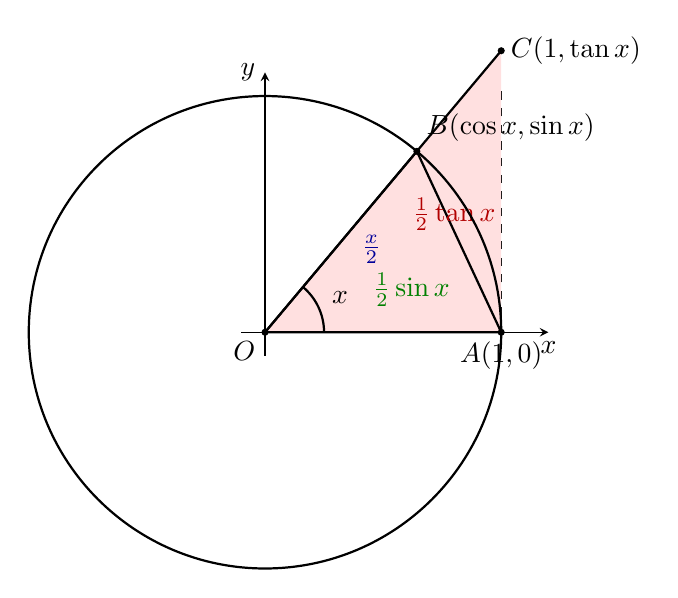
\begin{tikzpicture}[scale=3,>=stealth]
  % өнцөг
  \def\ang{50}

  % тэнхлэг, тойрог
  \draw[->] (-0.1,0) -- (1.2,0) node[below] {$x$};
  \draw[->] (0,-0.1) -- (0,1.1) node[left] {$y$};
 

  % цэгүүд
  \coordinate (O) at (0,0);
  \coordinate (A) at (1,0);
  \coordinate (B) at ({cos(\ang)},{sin(\ang)});
  \coordinate (C) at (1,{tan(\ang)});

  % сектор (нуугдмал өнгө)
  \fill[blue!12] (O) -- (A) arc (0:\ang:1) -- cycle;

  % гурвалжин OAB (дотоод)
  \fill[green!18] (O) -- (A) -- (B) -- cycle;

  % шүргэгч ба гурвалжин OAC (гадна)
  \draw[dashed] (1,0) -- (1,1.05);
  \fill[red!12] (O) -- (A) -- (C) -- cycle;

  % ирмэгүүд
  \draw[thick] (O) -- (A) -- (B) -- cycle;
  \draw[thick] (O) -- (C);

  % өнцгийн нум ба тэмдэглэгээ
  \draw[thick] (0.25,0) arc (0:\ang:0.25);
  \node at ({0.35*cos(\ang/2)},{0.35*sin(\ang/2)}) {$x$};

  % цэгүүдийн тэмдэглэгээ
  \fill (O) circle (0.015) node[below left] {$O$};
  \fill (A) circle (0.015) node[below] {$A(1,0)$};
  \fill (B) circle (0.015) node[above right] {$B(\cos x,\sin x)$};
  \fill (C) circle (0.015) node[right] {$C(1,\tan x)$};

  % тайлбар
  \node[green!50!black] at (0.62,0.18) {$\frac12\sin x$};
  \node[blue!60!black]  at (0.45,0.35) {$\frac{x}{2}$};
  \node[red!70!black]   at (0.80,0.50) {$\frac12\tan x$};
 \draw[thick] (0,0) circle (1);
\end{tikzpicture}
\end{center}

Талбайнууд:
\[
S_{\triangle OAB}=\frac12\sin x,\qquad
S_{\text{sector }OAB}=\frac{x}{2},\qquad
S_{\triangle OAC}=\frac12\tan x.
\]
Геометрийн хувьд $\triangle OAB$ нь сектороос бага, харин сектор нь $\triangle OAC$-аас бага тул
\[
\frac12\sin x\;<\;\frac{x}{2}\;<\;\frac12\tan x
\quad\Longrightarrow\quad
\sin x\;<\;x\;<\;\tan x.
\]
Өөрөөр 
\[
\cos x<\frac{\sin x}{x}<1 \qquad (0<x<\tfrac{\pi}{2})
\] гэж бичиж болно.
$x\to 0^+$ үед $\cos x\to 1$ тул Теорем \ref{ineqlim}.3-аар $\dfrac{\sin x}{x}\to 1$. $\dfrac{\sin x}{x}$ нь тэгш ($\sin(-x)/(-x)=\sin x/x$) тул $x\to 0-$ үед ч ижил дүгнэлт гарч,
\[
\lim_{x\to 0}\frac{\sin x}{x}=1.
\] Энэ хязгаарыг “I гайхамшигт хязгаар” гэж нэрлэдэг.
\end{example}
\begin{example}
    $(1+\dfrac{1}{2n})^n<2$ батал.

Бид семинар дээр $a>b>0$ ба $k\in\mathbb{N}$ бол 
\[
a^k \;<\;b^k+ k\,a^{\,k-1}(a-b)
\] байдгийг баталсан. Энд $a=1+\dfrac{1}{2n}  \;, \; b=1 \;, \;k=n+1$ гэвэл \[
\bigl( 1+\dfrac{1}{2n}\bigr) ^{\,n+1} \;<\; 1+(n+1)\,\bigl(1+\dfrac{1}{2n}\bigr)^{\,n}\Bigl(1+\dfrac{1}{2n}-1\Bigr)=1+(n+1)\,\bigl(1+\dfrac{1}{2n}\bigr)^{\,n}\cdot \frac{1}{2n}.
\]
Ингээд
\[
\bigl( 1+\dfrac{1}{2n}\bigr) ^{\,n+1}-(n+1)\,\bigl(1+\dfrac{1}{2n}\bigr)^{\,n}\cdot \frac{1}{2n}=\bigl(1+\dfrac{1}{2n}\bigr)^{\,n}\Bigl[1+\dfrac{1}{2n}-\dfrac{n+1}{2n}\Bigr] =\dfrac{1}{2}\bigl(1+\dfrac{1}{2n}\bigr)^{\,n}<1
\]
болно. Иймээс
\[
\Bigl(1+\frac{1}{2n}\Bigr)^{n} \;<\;2.
\]
батлагдав.
\end{example}
\begin{example}
    $\bigl(1+\dfrac{1}{n}\bigr)^n<\bigl(1+\dfrac{1}{n+1}\bigr)^{n+1}$ батал.

Өмнөх тэнцэтгэл бишид $a=1+\dfrac{1}{n}  \;, \; b=1\dfrac{1}{n+1} \;, \;k=n+1$ гэвэл батлагданa. 
\end{example}
\begin{example}[II гайхамшигт хязгаар]
     $\lim\limits_{n\to\infty}\Bigl(1+\dfrac{1}{n}\Bigr)^n$ дараалал нийлэхийг батал.

Өмнөх жишээнүүдээс $$4>(1+\dfrac{1}{2n})^{2n}>(1+\dfrac{1}{2n-1})^{2n-1}$$ гарах тул $\Bigl(1+\dfrac{1}{n}\Bigr)^n$ дараалал өсдөг дээрээсээ зааглагдсан дараалал байна. Иймд Теорем \ref{monton seq lim}-ээр хязгаартай. Энэ дараалалын хязгаарыг $e$ гэж нэрлэдэг.  $e\approx 2.7182818\dots$ байдаг.
     Энэ хязгаарыг “II гайхамшигт хязгаар” гэж нэрлэдэг.
\end{example}
\section{Семинар 7}
\begin{multicols}{2}
\begin{enumerate}
\item $\displaystyle \lim_{x\to -1} \frac{x^{2}-1}{x^{2}+3x+2}.$
\item $\displaystyle \lim_{x\to 5} \frac{x^{2}-25}{x-5}.$
\item $\displaystyle \lim_{x\to 2} \frac{x^{2}-5x+6}{x^{2}-12x+20}.$
\item $\displaystyle \lim_{x\to 1} \frac{2x^{3}-2x^{2}+x-1}{x^{3}-x^{2}+3x-3}.$
\item $\displaystyle \lim_{x\to -1} \frac{2x^{3}+2x^{2}+3x+3}{x^{3}+x^{2}+x+1}.$
\item $\displaystyle \lim_{x\to -3} \frac{x^{3}+5x^{2}+3x-9}{x^{3}+8x^{2}+21x+18}.$
\item $\displaystyle \lim_{x\to 0} \frac{x^{4}+x^{3}}{x^{4}-2x^{3}}.$
\item $\displaystyle \lim_{x\to a} \frac{x^{2}-(a+1)x+a}{x^{3}-a^{3}}.$
\item $\displaystyle \lim_{x\to 1} \Big(\frac{1}{1-x}-\frac{2}{1-x^{2}}\Big).$
\item $\displaystyle \lim_{x\to 0} \frac{\sqrt{x^{2}+1}-1}{\sqrt{x^{2}+16}-4}.$
\item $\displaystyle \lim_{x\to 0} \frac{\sqrt{1+x}-\sqrt{1-x}}{x}.$
\item $\displaystyle \lim_{h\to 0} \frac{\sqrt{x+h}-\sqrt{x}}{h}.$
\item $\displaystyle \lim_{x\to \infty} \big(\sqrt{x^{2}+1}-\sqrt{x^{2}-1}\big).$
\item $\displaystyle \lim_{x\to \pm\infty} (\sqrt{x^{2}+1}-x).$
\item $\displaystyle \lim_{x\to +\infty} x\, (\sqrt{x^{2}+1}-x).$
\item $\displaystyle \lim_{x\to 0} \frac{\sqrt[3]{1+x}-\sqrt[3]{1-x}}{x}.$
\item $\displaystyle \lim_{h\to 0} \frac{\sqrt[3]{x+h}-\sqrt[3]{x}}{h}.$
\item $\displaystyle \lim_{x\to -8} \frac{\sqrt{1-x}-3}{2+\sqrt[3]{x}}.$
\item $\displaystyle \lim_{x\to +\infty} \big(\sqrt[3]{x^{3}+x^{2}+1}-\sqrt[3]{x^{3}-x^{2}+1}\big).$
\item $\displaystyle \lim_{x\to \infty} \frac{1-3x}{2x+3}.$
\item $\displaystyle \lim_{x\to \infty} \frac{10x+5}{0.01\,x^{2}-6x}.$
\item $\displaystyle \lim_{x\to \infty} \frac{x^{3}-5x+2}{x+10^{10}}.$
\item $\displaystyle \lim_{x\to \infty} \frac{2x^{2}-3x-4}{\sqrt{x^{4}+1}}.$
\item $\displaystyle \lim_{x\to \infty} \frac{\sqrt{x}}{\sqrt{x+\sqrt{x}+\sqrt[4]{x}}}.$
\item $\displaystyle \lim_{x\to \infty} \big[\sqrt[3]{(x+1)^{2}}-\sqrt[3]{(x-1)^{2}}\big].$
\item $\displaystyle \lim_{x\to \infty} \frac{(x-1)^{3}}{2x^{3}+3x+1}.$
\item $\displaystyle \lim_{x\to \infty} \frac{x^{2}-5x+1}{3x+7}.$
\item $\displaystyle \lim_{x\to \infty} \frac{x}{\sqrt[3]{x^{3}+9}}.$
\item $\displaystyle \lim_{x\to \infty} \frac{\sqrt[3]{x^{2}+1}}{x+1}.$
\item $\displaystyle \lim_{x\to 0}\frac{\sin 3x}{x}$
\item $\displaystyle \lim_{x\to 0}\frac{\tan 5x}{\sin 2x}$
\item $\displaystyle \lim_{x\to 0}\frac{\tan 2x}{\tan 3x}$
\item $\displaystyle \lim_{x\to 0}\frac{\sin 4x}{\tan 3x}$
\item $\displaystyle \lim_{x\to 0}\frac{\tan 5x}{x}$
\item $\displaystyle \lim_{x\to 0}\frac{1-\cos x}{x^{2}}$
\item $\displaystyle \lim_{x\to 0}\frac{\tan x-\sin x}{x^{3}}$
\item $\displaystyle \lim_{x\to 0}\frac{1-\cos 2x}{x^{2}}$
\item $\displaystyle \lim_{x\to 0}\frac{\ln(1+x)}{x}$
\item $\displaystyle \lim_{x\to 0}\frac{\ln(1+2x)}{x}$
\item $\displaystyle \lim_{x\to 0}\frac{\ln(1+x)-x}{x^{3}}$
\item $\displaystyle \lim_{x\to 0}\frac{e^{x}-1-x}{x^{2}}$
\item $\displaystyle \lim_{x\to 0}\frac{(1+x)^{a}-(1+x)^{b}}{x}$
\item $\displaystyle \lim_{x\to 0}\frac{(1+x)^{n}-1}{x}$
\item $\displaystyle \lim_{x\to 0}\frac{(1+7x)^{9}-1-63x}{x^{2}}$
\item $\displaystyle \lim_{x\to 0}\frac{e^{3x}-1}{x+x^{2}}$
\end{enumerate}
\end{multicols}
\section*{Хязгаар сэдвийн даалгавар}
\begin{enumerate}
\item Хязгаарыг тодорхойлолтын дагуу шалга.
\begin{multicols}{2}
\begin{enumerate}
\item $\lim\limits_{x\to 2}\sqrt{x}=\sqrt{2}$ 
\item $\lim\limits_{x\to 2}(3x+5)=11$
\item $\lim\limits_{n\to +\infty}\dfrac{n^2+2n+1}{n^2+n+1}=1$
\item $\lim\limits_{n\to \infty}\dfrac{n}{n+1}=1$
\end{enumerate}
\end{multicols}
\item Хязгаарыг бод.
\begin{multicols}{2}
\begin{enumerate}
\item $\lim\limits_{x\to 1}\dfrac{x^2-1}{x-1}$
\item $\lim\limits_{x\to 4}\dfrac{\sqrt{x}-2}{x-4}$
\item $\lim\limits_{x\to \infty}\dfrac{3x^2+2}{5x^2-7}$
\item $\lim\limits_{x\to \infty}\dfrac{\sqrt{x^2+3}}{x}$
\item $\lim\limits_{x\to 0^+}\dfrac{1}{x}$
\item $\lim\limits _{x\to 1} \dfrac{x^{n+1}-(n+1)x+n}{(x-1)^2}$ 
\item $\lim\limits _{x\to 1} \dfrac{m}{1-x^m}-\dfrac{n}{1-x^n}$
\item $\lim\limits _{x\to +\infty} \dfrac{\sqrt{x+\sqrt{x+\sqrt{x}}}}{\sqrt{x+1}}$
\item $\lim\limits _{x\to +\infty} \dfrac{\sqrt{x}+\sqrt[3]{x}+\sqrt[4]{x}}{\sqrt{2x+1}}$ 
\item $\lim\limits _{x\to 4} \dfrac{\sqrt{1+2x}-3}{\sqrt{x}-2}$
\item $\lim\limits _{x\to 8} \dfrac{\sqrt{1+x}-3}{\sqrt[3]{x}-2}$
\item $\lim\limits_{x\to \infty}\dfrac{2x+3}{5x-1}$
\item $\lim\limits_{x\to -\infty}\dfrac{x^2+1}{2x^2-3}$
\item $\lim\limits_{x\to \infty}\dfrac{2x^3-1}{x^3+5}$
\item $\lim\limits_{x\to 0}\dfrac{\sqrt{1+x}-1}{x}$
\item $\lim\limits_{x\to 0}\dfrac{\ln(1+2x)}{x}$
\item $\lim\limits_{x\to \infty}\dfrac{\sqrt{x^2+5x}}{x}$
\end{enumerate}
\end{multicols}
\item I гайхамшигт хязгаар хэрэглэн хязгаарыг бод.
\begin{multicols}{2}
\begin{enumerate}
\item $\lim\limits_{x\to 0}\dfrac{\sin x}{x}$
\item $\lim\limits_{x\to 0}\dfrac{1-\cos x}{x^2}$
\item $\lim\limits_{x\to 0}\dfrac{\tan x}{x}$
\item $\lim\limits_{x\to 0}\dfrac{\sin(2x)}{x}$
\item $\lim\limits_{x\to 0}\dfrac{\arctan x}{x}$
\item $\lim\limits_{x\to 0}\dfrac{1-\cos(3x)}{x^2}$
\item $\lim\limits_{x\to 0}\dfrac{\sin x - x}{x^3}$
\item $\lim\limits_{n\to \infty}\dfrac{\sin x}{x}$
\item $\lim\limits_{x\to 0}\dfrac{\tan(5x)}{x}$
\item $\lim\limits_{x\to 0}\dfrac{\arcsin x}{x}$
\item $\lim\limits_{x\to 0}\dfrac{\sin x}{1-\cos x}$
\item $\lim\limits_{x\to \frac{\pi}{6}}\dfrac{2\sin x-1}{1-2\cos 2x}$
\end{enumerate}
\end{multicols}
\item  Дараалалын хязгаар бод.
\begin{multicols}{2}
\begin{enumerate}
\item $\lim\limits_{n\to \infty}\dfrac{1}{n}$
\item $\lim\limits_{n\to \infty}\dfrac{2^n}{3^n}$
\item $\lim\limits_{n\to \infty}\dfrac{n!}{n^n}$
\item $\lim\limits_{n\to -\infty}(1+\dfrac{1}{n})^n$
\item $\lim\limits_{n\to \infty}\sqrt[n]{2}$
\item $\lim\limits_{x\to \infty}\sqrt[n]{n}$
\item $\lim\limits_{n\to \infty}\dfrac{n}{2^n}$
\item $\lim\limits_{n\to \infty}\dfrac{2^n}{n!}$
\item $\lim\limits_{n\to \infty}\sqrt[n]{n^2+3}$
\item $\lim\limits_{n\to \infty}\left(1+\dfrac{2}{n}\right)^n$
\item $\lim\limits_{n\to \infty}\dfrac{1}{\sqrt{n}}$
\item $\lim\limits_{n\to \infty}\dfrac{\ln n}{n}$
\item $\lim\limits_{n\to \infty}\dfrac{n}{\ln n}$
\item $\lim\limits_{n\to \infty}\sqrt[n]{3^n+5}$
\item $\lim\limits_{n\to \infty}\dfrac{\sin(1/n)}{1/n}$
\item $\lim\limits_{n\to \infty}(1+\dfrac{1}{n})^{2n}$
\item $\lim\limits_{n\to \infty}\dfrac{(n+1)!}{(n!)^2}$
\item $\lim\limits_{n\to \infty}\dfrac{n^k}{e^n}$ ($k$ тогтмол)
\item $\lim\limits_{n\to \infty}\dfrac{e^n}{n^k}$ ($k$ тогтмол)
\item $\lim\limits_{n\to \infty}\sqrt[n]{n!}$
\item $\lim\limits_{n\to \infty}\dfrac{1+2+\cdots+n}{n^2}$
\item $\lim\limits_{n\to \infty}\dfrac{\sin n}{n^2}$
\end{enumerate}
\end{multicols}
\item II гайхамшигт хязгаар хэрэглэн хязгаарыг бод.
\begin{multicols}{2}
\begin{enumerate}
\item $\lim\limits_{x\to \infty}\dfrac{\ln x}{x}$
\item $\lim\limits_{x\to 1}\dfrac{\ln x}{x-1}$
\item $\lim\limits_{x\to 0}\dfrac{e^{2x}-1}{x}$
\item $\lim\limits_{x\to \infty}\left(1+\dfrac{2}{x}\right)^{3x}$
\item $\lim\limits_{x\to \infty}\dfrac{\ln(x^2+1)}{\ln x}$
\item $\lim\limits_{x\to \infty}\dfrac{x^3}{e^x}$
\item $\lim\limits_{x\to 0}\dfrac{e^x-1}{x}$
\item $\lim\limits_{x\to 0}\dfrac{\ln(1+x)}{x}$
\item $\lim\limits_{x\to \infty}\dfrac{e^x}{x^3}$
\item $\lim\limits_{x\to \infty}\dfrac{\ln x}{\sqrt{x}}$
\end{enumerate}
\end{multicols}
\end{enumerate}
